\subsection{Classifier: Diagonal Covariance (Per-Class)}

% \begin{figure}[H]
%     \centering
%     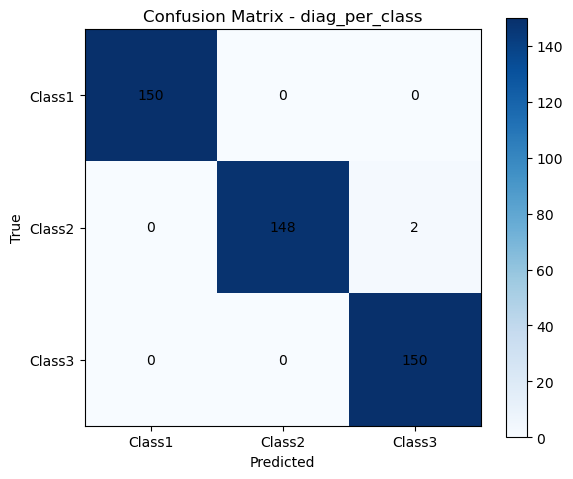
\includegraphics[width=0.75\linewidth]{images/LS_Group04_images/03_diag_per_class/01_confusion_matrix.png}
%     \caption{Confusion Matrix for Diagonal Covariance (Per-Class) (Linearly Separable Data)}
% \end{figure}

\begin{table}[H]
\centering
\caption{Confusion Matrix for Diagonal Covariance (Per-Class) (Linearly Separable Data)}
\label{tab:confmat_LSD_Diagonal Covariance (Per-Class)}
\begin{tabular}{|c|c|c|c|}
\hline
\textbf{Actual $\backslash$ Predicted} & \textbf{Class 1} & \textbf{Class 2} & \textbf{Class 3} \\
\hline
\textbf{Class 1} & 150 & 0   & 0   \\
\textbf{Class 2} & 0  & 148 & 2   \\
\textbf{Class 3} & 0   & 0   & 150 \\
\hline
\end{tabular}
\end{table}


\begin{table}[H]
\centering
\caption{Performance Metrics - Diagonal Covariance (Per-Class)}
\begin{tabular}{lcccc}
\toprule
\textbf{Class} & \textbf{Precision} & \textbf{Recall} & \textbf{F1-Score} & \textbf{Support} \\
\midrule
Class 1 & 1.0000 & 1.0000 & 1.0000 & 125 \\
Class 2 & 1.0000 & 1.0000 & 1.0000 & 125 \\
Class 3 & 1.0000 & 1.0000 & 1.0000 & 125 \\
\midrule
\textbf{Accuracy} & \multicolumn{4}{c}{1.0000} \\
\textbf{Mean Precision} & \multicolumn{4}{c}{1.0000} \\
\textbf{Mean Recall} & \multicolumn{4}{c}{1.0000} \\
\textbf{Mean F1 Score} & \multicolumn{4}{c}{1.0000} \\
\bottomrule
\end{tabular}
\end{table}

\textbf{Inferences:} Allowing per-class diagonal covariance still perfectly classifies this dataset, as features vary independently along axes with clear class separation.

\begin{figure}[H]
    \centering
    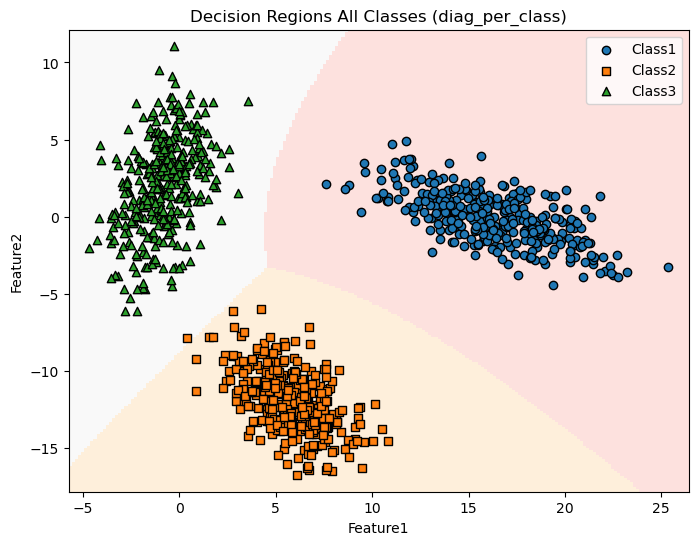
\includegraphics[width=\linewidth]{images/LS_Group04_images/03_diag_per_class/05_decision_region_all.png}
    \caption{Decision Region Plot (All Classes) - Diagonal Covariance (Per-Class)}
\end{figure}

\subsubsection{Decision Region Plots Between Class Pairs (LS Dataset, Diagonal Covariance (Per-Class))}


\begin{figure}[H]
    \centering
    \begin{minipage}{0.32\linewidth}
        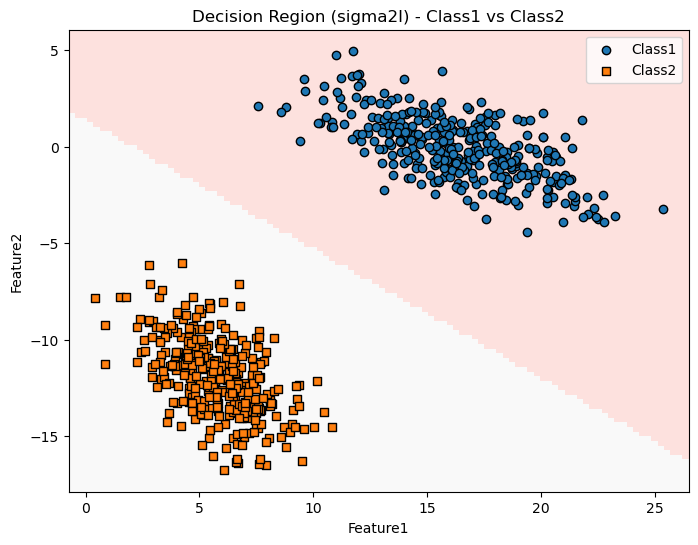
\includegraphics[width=\linewidth]{images/LS_Group04_images/01_sigma2i/02_decision_region_c1_c2.png}
        \caption*{Class 1 vs Class 2}
    \end{minipage}
    \hfill
    \begin{minipage}{0.32\linewidth}
        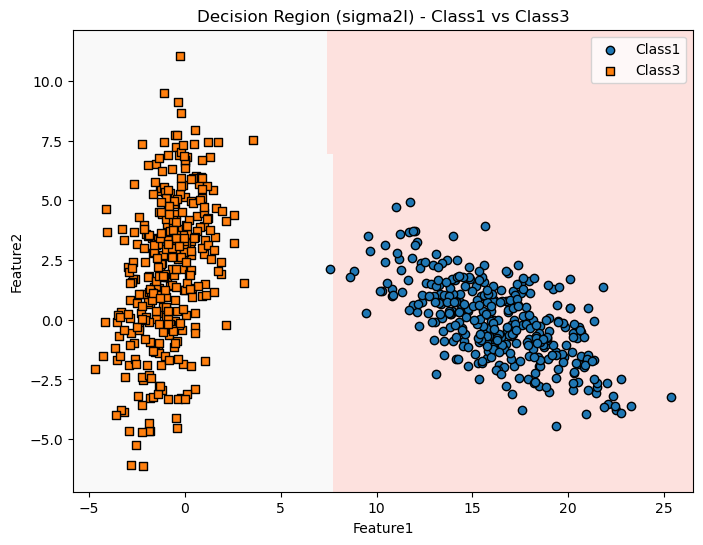
\includegraphics[width=\linewidth]{images/LS_Group04_images/01_sigma2i/03_decision_region_c1_c3.png}
        \caption*{Class 1 vs Class 3}
    \end{minipage}
    \hfill
    \begin{minipage}{0.32\linewidth}
        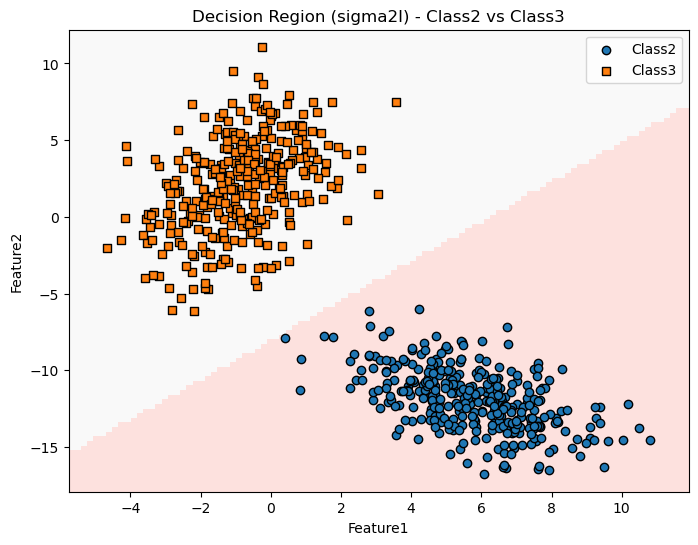
\includegraphics[width=\linewidth]{images/LS_Group04_images/01_sigma2i/04_decision_region_c2_c3.png}
        \caption*{Class 2 vs Class 3}
    \end{minipage}
    \caption{Decision Region Plots (Training data points superimposed) between class pairs for Diagonal Covariance (Per-Class) on LS dataset}
\end{figure}